% vim:tw=80:filetype=on:filetype=tex
\ignore{
\wfigure[Graphs/xdd.pdf,{\figtitle{\CChell{} performance: xdd}},fig:xdd]
}

\section{Results: \CChell{}}
\label{sec:results-chell}

In this section we evaluate \CChell{}'s latency and bandwidth using a
collection of micro- and macro-benchmarks.  


\subsection{Experimental setup}
\label{sec:setup}

We use the same system for this evaluation as we did in
section~\ref{sec:results-quill}. We use a 1~GB file to test
\CChell{} performance. To compare it with Linux page cache, we also ran the
same tests directly on the backing store device and disabled any DIRECT I/O
option to make sure page cache was used.  We set the cache size to 8~GB and use
a 120~GB SSD as backing store device, mounted with an Ext4 file system.  We
repeated each test three times to make sure both \CChell{} and page cache warm.

\subsection{Microbenchmarks}
\label{sec:microbenchmark}

\begin{figure}
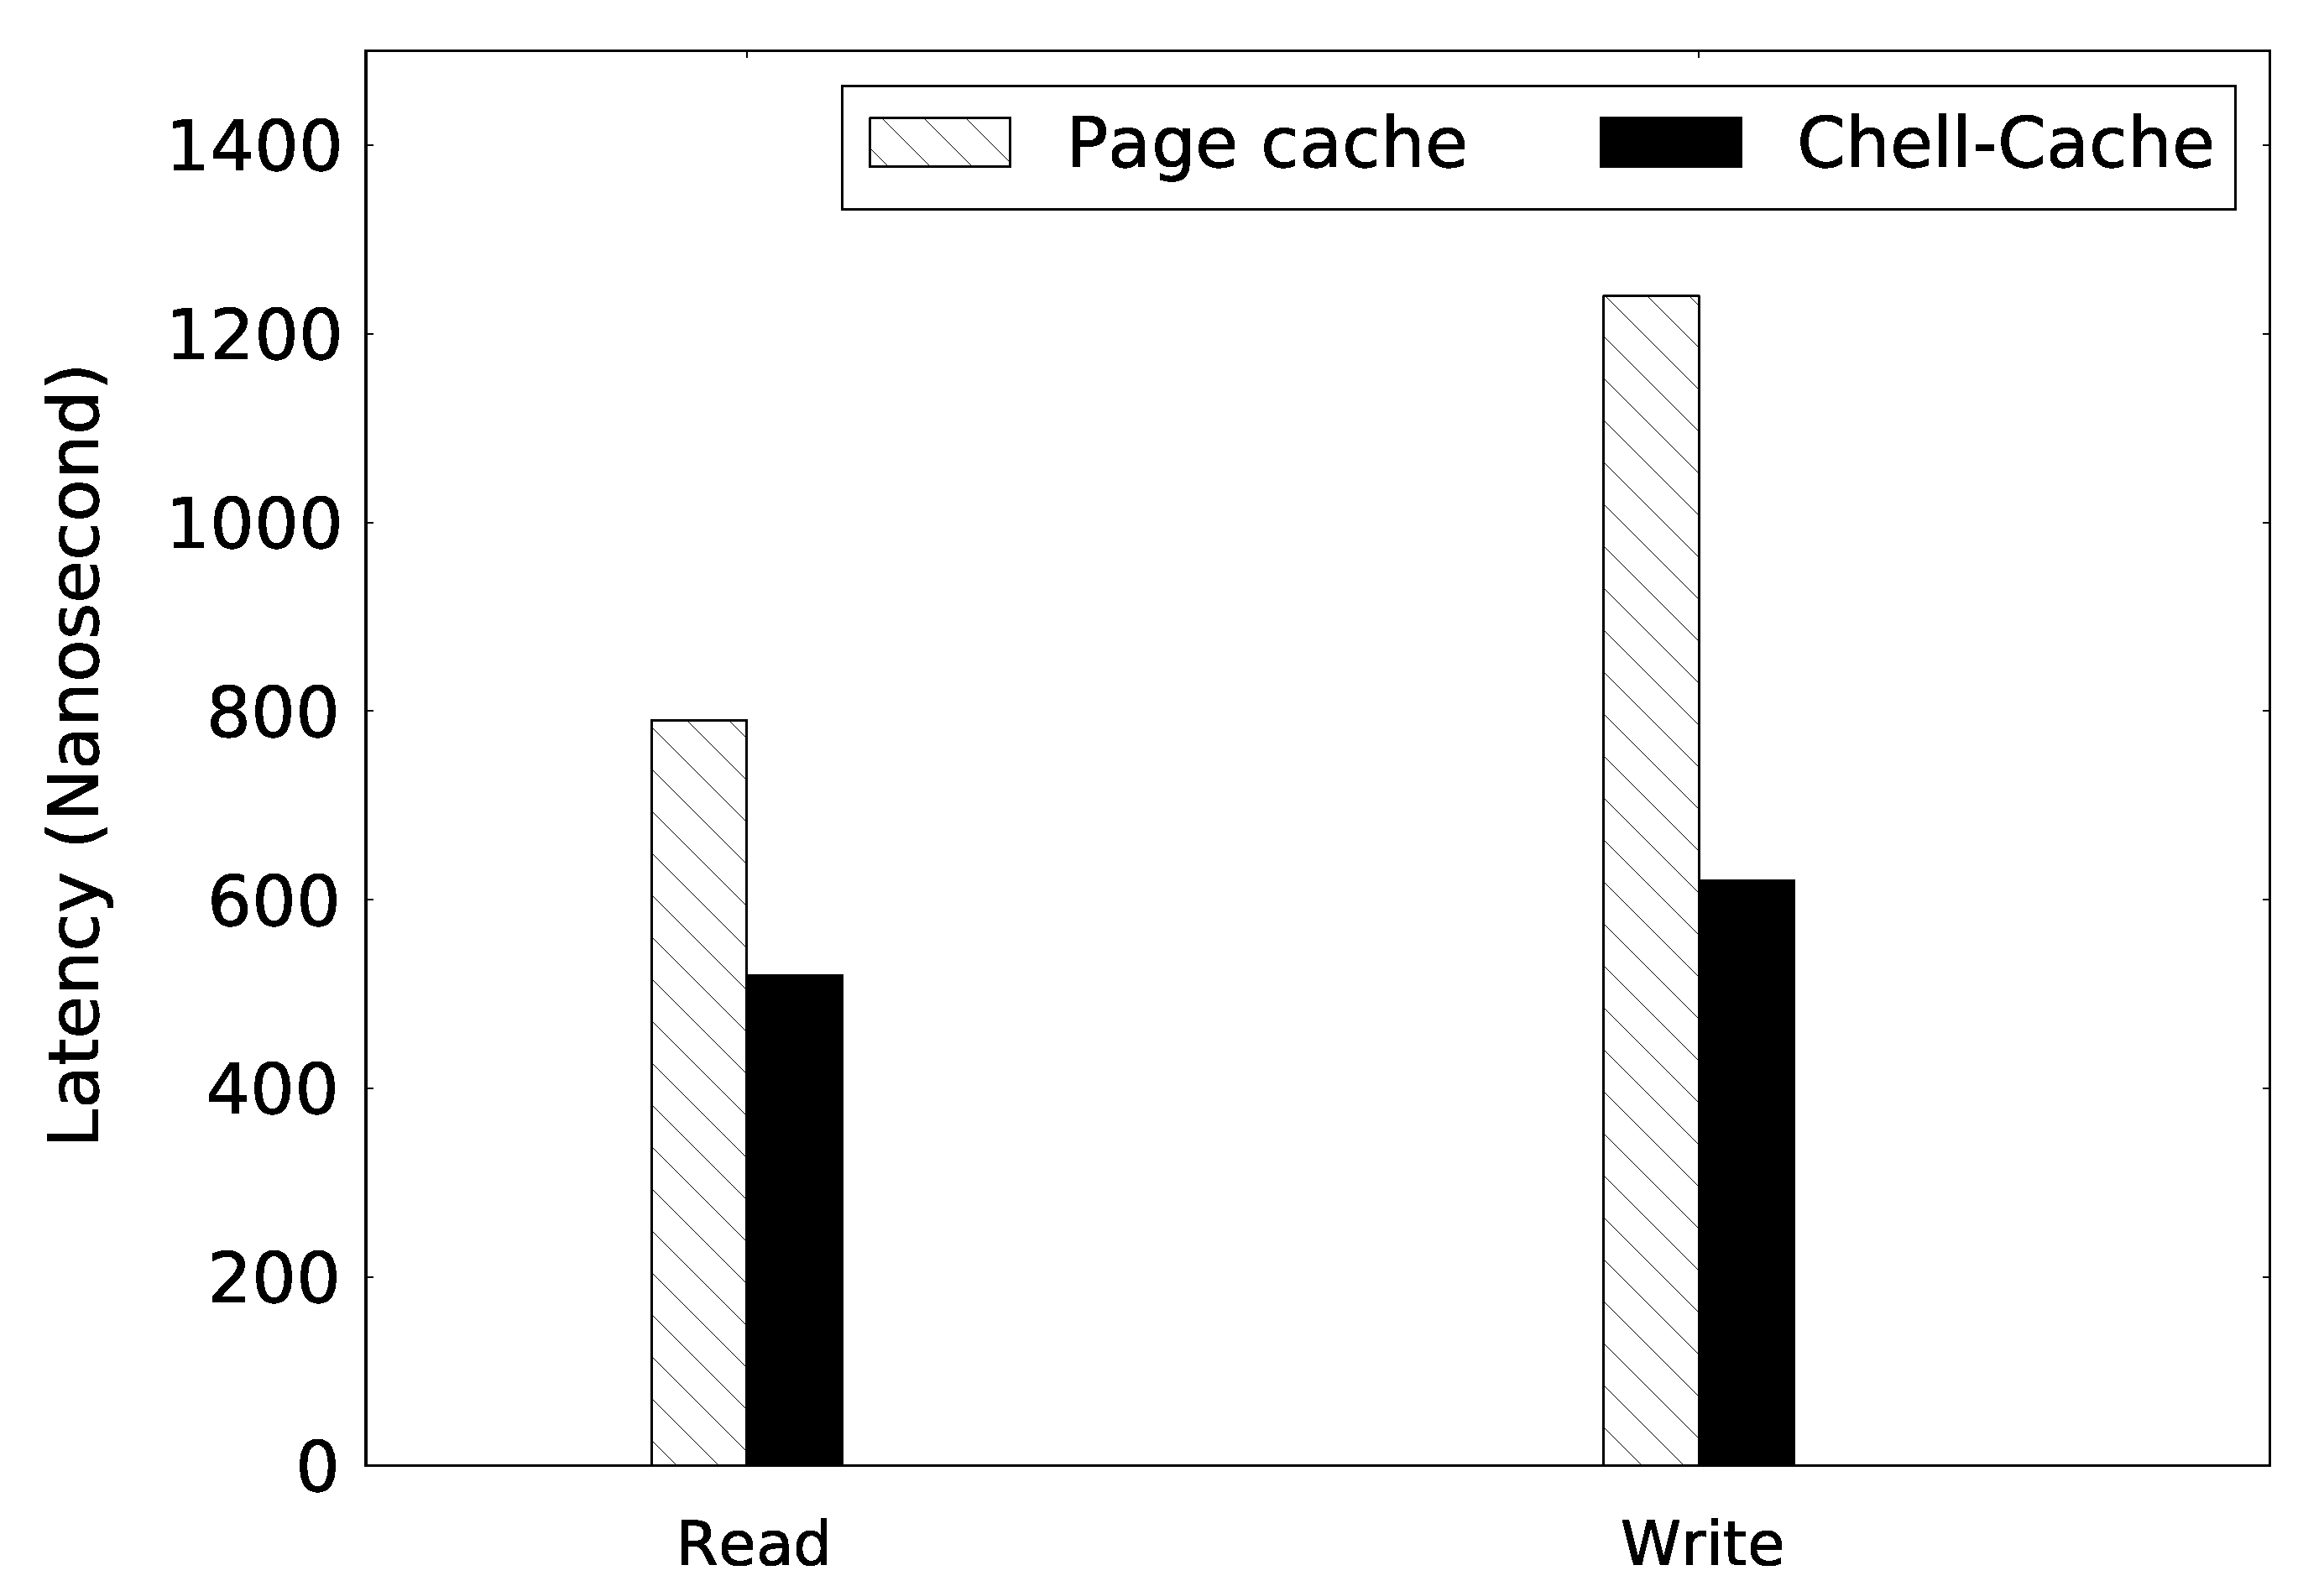
\includegraphics[width=\linewidth]{Graphs/latency.pdf}
\centering
\caption{\CChell{} 4KB access latency}
\label{fig:chell-latency}
\end{figure}

\wfigure[Graphs/xdd.pdf,{\figtitle{\CChell{} performance: xdd}},fig:xdd]

To evaluate \CChell{}'s performance characteristics we used a combination of
custom-built microbenchmarks, XDD~\cite{xdd}, and IOZone~\cite{iozone}.

Figure~\ref{fig:chell-latency} shows the 4~kB access latency of \CChell{}.
Accessing the cache pages
directly from the user space allows \CChell{} to reduce read/write operation
latency.  To perform a 4~kB read operation, \CChell{} takes
about 520~ns on average, while a 4~kB read from page cache takes about 790~ns.
For 4~kB write, \CChell{} takes 620~ns, and page cache takes 1240~ns.

\CChell{} reduces latency by 35\% for 4~kB reads and 50\% for 4~kB writes, because entering the kernel
takes a significant part
of the whole operation for small memory accesses. By pypassing the kernel,
\CChell{} eliminates this overhead. 

Figure~\ref{fig:xdd} compares the bandwidth of \CChell{} and page cache for sequential and
random 4~kB access in three different read/write combinations: 0\% writes
(read), 50\% writes (50/50) and 99\% writes (write).

For single-threaded bandwidth, \CChell{} outperforms the page cache 
all three workloads, with improvements ranging from 32\% for random read to
178\% for sequential write.  With four threads,
\CChell{} outperforms page cache by 47\% for random read up to 245\% for sequential writes.
With 16 threads, \CChell{}'s sequential access performance is lower than it is with
four threads.  We suspect this is \andiry{This doesn't make any sense.  Why would this be? because multiple threads accessing
the same memory block limits bandwidth}, but \CChell{} still outperforms page
cache by \andiry{X\%}.  For random accesses with 16 threads, \CChell{}
outperforms the page cache 63\% for reads and 283\% for
writes.

%\wfigure[Graphs/xdd.pdf,{\figtitle{\Chell{} performance: xdd}}
%,fig:xdd]

\ignore{
\begin{figure*}
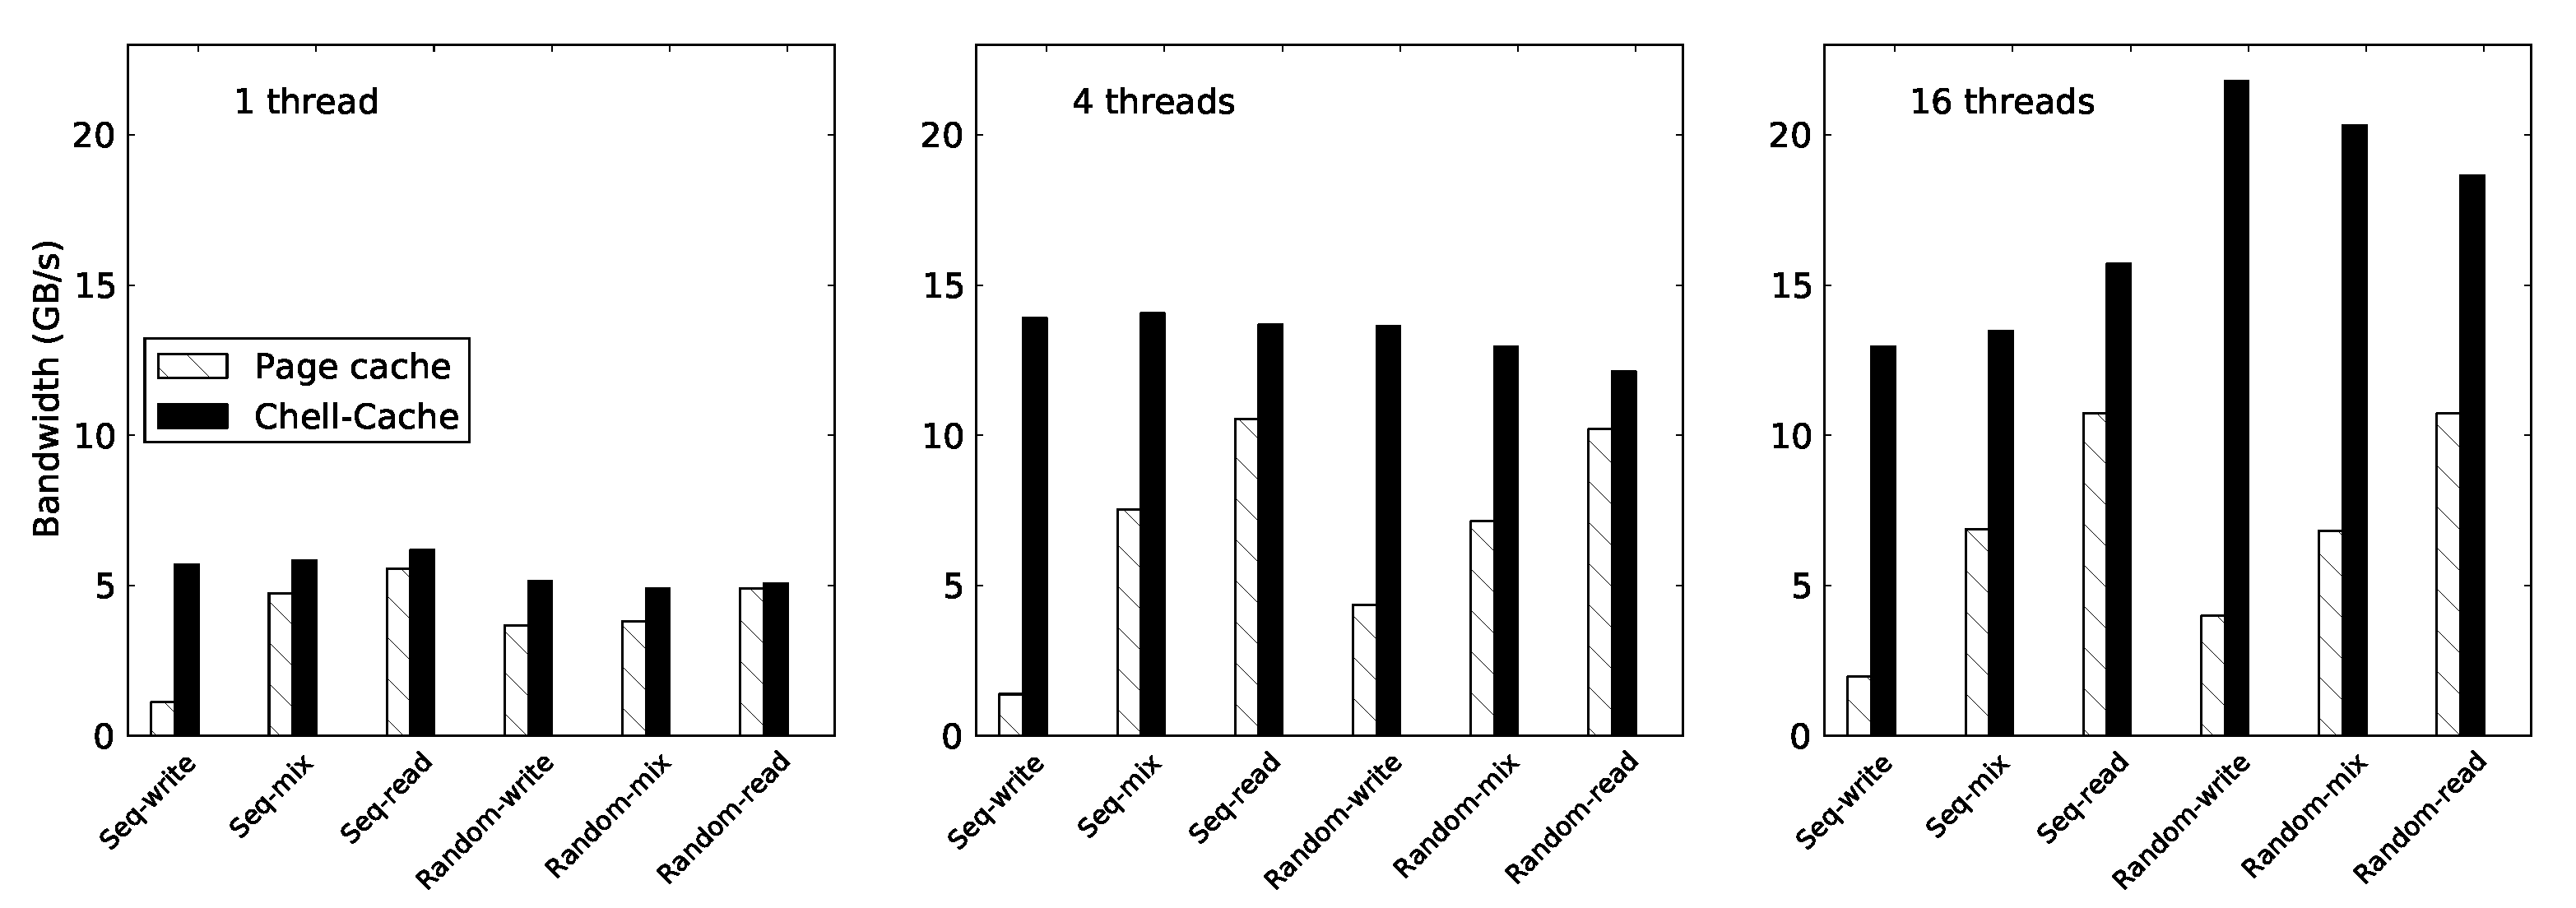
\includegraphics[width=\textwidth]{Graphs/xdd.pdf}
\vspace*{-5mm}\caption{\CChell{} performance: xdd}
\label{fig:xdd}
\end{figure*}
}

IOzone~\cite{IOzone} is a filesystem benchmark tool that provides many different types of 
operation patterns. We use it to confirm the results from xdd and measure a wider range of access patterns.  We evaluated the performance for read, write,
re-read, re-write, random read/write, read backwards, record rewrite and
strided read.

Figure~\ref{fig:iozone} shows the bandwidth of \CChell{} and page cache
for different IOzone tests, with 4~kB access size and 1~GB file size.
\CChell{} improves bandwidth over page cache in all test cases,
from 29\% (random read) to 103\% (random write).

\cfigure[Graphs/iozone.pdf,{\figtitle{\CChell{} performance: IOzone}},fig:iozone]

When an application appends to a file, \CChell{} needs to notify the file system
on the backing store device that the metadata of the file has changed. There
are two ways to do this: one is to simply send the write request to the file
system, and the other is to call \texttt{fallocate()} to allocate space for
the file on the backing store device, then write the data to NVMM cache.

\cfigure[Graphs/fallocate.pdf,{\figtitle{\CChell{} fallocate() performance}},fig:fallocate]

Figure~\ref{fig:fallocate} shows the impact of \texttt{fallocate()}
to \CChell{} performance with different request sizes. As we expect, for small
request (less than 32~kB), the overhead of \texttt{write()} is smaller than 
\texttt{fallocate()} and copy data to cache.  For requests equal to or larger
than 32~kB, using \texttt{fallocate()} is more efficient.  In \CChell() we use
32~kB as a threshold to trigger \texttt{fallocate()} for file appendings.

%\cfigure[Figures/blank.pdf,{\figtitle{\Chell{} Bandwidth}:
%A graph shows the bandwidth results of \Chell{}.}
%,fig:bankshotbandwidth]


\subsection{MacroBenchmarks}
\label{sec:macrobenchmark}

\ignore{To show the macro benchmark performance.}

\ignore{You can't reuse the same text here as you had in quill result section. It'll annoy the reader.  You can just say you used the same workload that we described earlier, but you still need to fix the earlier description (see notes there).}

We use Berkeley-DB Btree application to evaluate the performance of
\CChell{} with real applications.
The application runs with a
single thread, two threads, four threads, or eight threads. Berkeley-DB
uses multiple threads to perform database lookup and update operations.

Figure~\ref{fig:bdb-chell} shows the performance of Berkeley-DB Btree
application on \CChell{}.  \Chell{} boosts the
throughput by 3.7\x{} to 4.8\x{} compare with page cache, and close to the
performance of Berkeley-DB Btree running directly on PMFS.

Berkeley-DB calls \texttt{fdsync()} for each
write operation to sync
file data to storage devices to ensure the data persistency.
For each \texttt{fdsync()}, \lib{} flushes the affected cachelines, while \drv{} ensures the cache metadata remains consistent in the event of a system crash.  This significantly reduces the sync latency and improves application-level performance.

\cfigure[Graphs/bdb-chell.pdf,{\figtitle{\CChell{} performance: Berkeley-DB}},fig:bdb-chell]

We also run Filebench~\cite{filebench} workloads with \CChell{}. Filebench
is a file system and storage benchmark, it includes several useful
macro-benchmarks to emulate real applications. In the test we show the
normalized performance of \CChell{} comparing to page cache, with different
average file size.

Figure~\ref{fig:filebench} shows the performance of \CChell{} on filebench.
We choose three workloads: fileserver, webserver and varmail.
The fileserver wrokload creates files, append to them, read them and
then close and delete.
With average file size of 128~kB, \CChell{} gets 77\% performance
of page cache. This is because we \texttt{mmap} files with 2~MB chunk,
and files less than 2~MB are not memory mapped to user space, and we pay
the overhead of going to kernel space. Also, as fileserver creates new files,
all the data go to the backing store device and undermines the \CChell{}
performance. When the average file size increases, \CChell{} shows better
performance than page cache: for 512~kB files it ourperforms page cache
by 31\% and for 2~MB files the performance gain is 91\%. Similarly, with
webserver workload, \CChell{} outperforms page cache by 28\% for average
file size of 2~MB; with varmail workload, \CChell[] performs even better,
improves the performance from 82\% (512~kB) to 226\% (2~MB) over page cache.
This is because varmail workload uses \texttt{fsync()} to make file
persistent, and with \CChell{} the \texttt{fsync()} is much more efficient.

\cfigure[Graphs/filebench.pdf,{\figtitle{\CChell{} performance:
Filebench}},fig:filebench]


